\begin{figure}[h!]

\centering
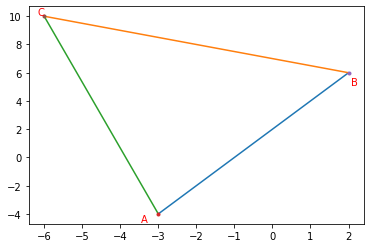
\includegraphics[width=0.5\textwidth]{solutions/1/1/4/Figure_1}
\caption{Right Angled Triangle}
\label{eq:solutions/1/1/4/fig:triangle}
\end{figure}
Say there exists two points $\textbf{P}(x_1, y_1)$ and $\textbf{Q}(x_2, y_2)$. The distance between the points is:
% Equation of y axis is 
\begin{align}
    \textbf{Z = P - Q}
\end{align}
Distance between \textbf{P} and \textbf{Q} is given by 
% For   $\Vec{
% 1 & -2 \\
% }x = 4$ (at y axis meet)
\begin{align}
||\textbf{Z}|| = \norm{\textbf{P-Q}}
\end{align}
% \begin{align}
% d = 
% \end{align}
Let $\textbf{P} = (-3, -4)$, $\textbf{Q} = (2, 6)$ and $\textbf{R} = (-6, 10)$.
\begin{enumerate}
    \item Distance between \textbf{P} and \textbf{Q} is 
\begin{align}
\norm{\textbf{P-Q}} = \sqrt{(-3-2)^2+(-4-6)^2}
=\sqrt{125}
\end{align}
\item Distance between \textbf{Q} and \textbf{R} is 
\begin{align}
\norm{\textbf{Q-R}} = \sqrt{(2-(-6))^2+(6-10)^2}
=\sqrt{80}
\end{align}
\item Distance between \textbf{P} and \textbf{R} is 
\begin{align}
\norm{\textbf{P-R}} = \sqrt{(-3-(-6))^2+(-4-10)^2}
=\sqrt{205}
\end{align}
\end{enumerate}
Here, the largest distance is $\sqrt{205}$. To be vertices of a right angled triangle, we should have 
\begin{align}
  \norm{\textbf{P-Q}}^2 + \norm{\textbf{Q-R}}^2 = \norm{\textbf{R-P}}^2
\end{align}
\begin{align}
  (\sqrt{205})^2 = (\sqrt{125})^2 + (\sqrt{80})^2
\end{align}
\begin{align}
  205 = 205
\end{align}
So, the condition is satisfied. 
So, using Baudhayana's theorem, it is proved that 3 points given are vertices of a right angled triangle. 
Now, for orthogonality, 
\begin{align}
    (\vec{P-Q})^T(\vec{Q-R}) = 0
\end{align}
We have 
\begin{enumerate}
    
    \item \begin{align}
    \vec{P-Q} = (2-(-3), 6-(-4))
\\
\vec{P-Q} = \myvec{
5\\
10 
}
\end{align}
    \item \begin{align}
    \vec{Q-R} = (2-(-6), 6-10)
\\
\vec{Q-R} = \myvec{
8\\
-4 
}
\end{align}
\item \begin{align}
    \vec{P-R} = (-3-(-6), -4-10)
\\
\vec{P-R} = \myvec{
3\\
-14 
}
\end{align}
\end{enumerate}
% We have 
% % \overrightarrow{\text {PQ}}
% \begin{align}
% \textbf{P}
% \\
%          \textbf{X}=(2-(-3), 6-(-4))
%  \\\textbf{X}= \myvec{
% 5\\
% 10 
% }
% \end{align}
% \overrightarrow{\text {QR}}
% Assuming Y is the vector, connecting Q and R. 
% \begin{align}
% \textbf{Y} = $$Q-R$$
% \\
%          \textbf{Y}=(2-(-6), 6-10)
%  \\\textbf{Y}= \myvec{
% 8\\
% -4 
% }
% \end{align}
% Assuming Z is the vector connecting P and R. 
% \begin{align}
% \textbf{Z} = $$P-R$$
% \\
%          \textbf{Z}=(-3-(-6), -4-10)
%  \\\textbf{Z}= \myvec{
% 3\\
% -14 
% }
% \end{align}
For orthogonality, product of transpose of one point and other must be 0. 
Here, checking for 
\begin{align}
    \myvec{
5\\
10 
}^T\myvec{ 8\\
-4
} =  \myvec{
5\\
10
}^T \myvec{
8 \\ -4
}=0
\end{align}
Hence, using orthogonality, it is proved that the points form a right angled triangle. 

%\section{figure}

Figure \ref{eq:solutions/1/1/4/fig:triangle} Right anlged triangle where A=P and B=Q and C=R


